

\chapter{Les technologies utilisées}

\section{Un bref historique du développement d'applications mobiles}
Le développement d'applications mobiles est l'acte ou le processus par lequel une application est développée pour les appareils mobiles. Ces applications peuvent être préinstallées sur les téléphones au cours de la fabrication ou accessibles via un navigateur Web \cite{noauthor_mobile_2019}. Toutefois, au cours de la dernière décennie \cite{leler_whats_2017}, des développeurs tiers ont été capables de créer des applications mobiles. Cependant, en raison de la concurrence intense dans les logiciels mobiles et des modifications apportées à chacune des plateformes, ces développeurs doivent prendre en compte un large éventail de tailles d'écran, de spécifications matérielles et de configurations.\\
\tab Le développement d'applications mobiles est un domaine d'activité relativement récent. il n’est donc pas surprenant que les outils évoluent encore.
\newpage

\subsection{Les kits de développement de plate-forme (Platform SDKs)}
Le SDK Apple iOS est sorti en 2008 et le SDK Google Android en 2009. Ces deux SDK étaient basés sur des langages différents: Objective-C et Java, respectivement.
Votre application communique avec la plateforme pour créer des widgets ou accéder à des services tels que la caméra. Les widgets sont rendus dans un canevas d’écran et les événements sont renvoyés aux widgets. C'est une architecture simple, mais vous devez créer des applications séparées pour chaque plate-forme car les widgets sont différents, sans parler des langues natives\cite{leler_whats_2017}.

\begin{figure}[h]
	\begin{center}
		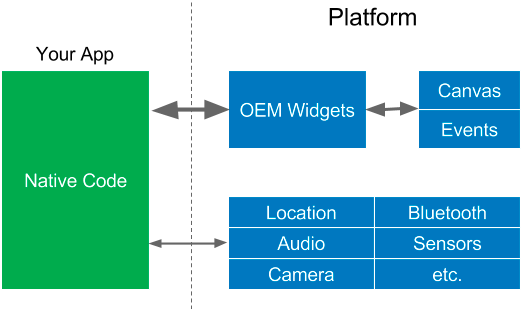
\includegraphics[width=10cm]{Images/chapter2/platform_sdk.png}
		\caption{{\footnotesize Architecture du développement mobile a l'aide des SDK\cite{leler_whats_2017}}}
	\end{center}
\end{figure}

\subsection{Vues Web (WebViews)}
Les premiers frameworks multi-plateformes étaient basés sur JavaScript et WebViews. Les exemples incluent une famille de frameworks liés: PhoneGap, Apache Cordova, Ionic, etc. Avant de publier leur SDK iOS, Apple avait encouragé les développeurs tiers à créer des applications Web pour iPhone. Il était donc évident de créer des applications multiplates-formes à l'aide de technologies Web.

\begin{figure}[h]
	\begin{center}
		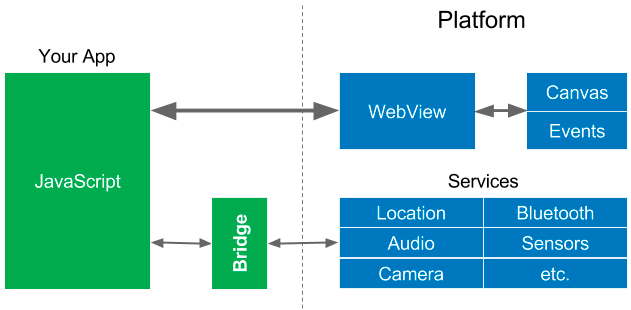
\includegraphics[width=11cm]{Images/chapter2/webview.png}
		\caption{{\footnotesize Architecture du développement mobile a l'aide des WebViews\cite{leler_whats_2017}}}
	\end{center}
\end{figure}

Votre application crée du HTML et l'affiche dans une vue Web sur la plateforme. Notez qu'il est difficile pour des langages tels que JavaScript de parler directement au code natif (comme les services), de sorte qu'ils passent par un «pont» qui fait que le contexte bascule entre le domaine JavaScript et le domaine natif. Comme les services de plate-forme ne sont généralement pas appelés très souvent, cela n’a pas causé trop de problèmes de performances\cite{leler_whats_2017}.

\subsection{Vues réactives (Reactive Views)}
Les infrastructures Web réactives telles que ReactJS (et d'autres) sont devenues populaires, principalement parce qu'elles simplifient la création de vues Web grâce à l'utilisation de modèles de programmation empruntés à la programmation réactive. En 2015, React Native a été créé pour apporter les nombreux avantages des vues réactives aux applications mobiles.\\

\begin{figure}[h]
	\begin{center}
		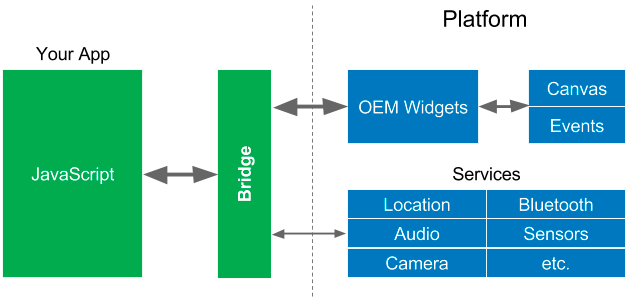
\includegraphics[width=11cm]{Images/chapter2/reactive_views.png}
		\caption{{\footnotesize Architecture du développement mobile a l'aide des Reactive Views\cite{leler_whats_2017}}}
	\end{center}
\end{figure}

\begin{wrapfigure}[8]{r}{2cm}
	
\includegraphics[width=2cm]{Images/chapter2/react_native_logo.png}
	\caption{{\footnotesize Logo de React Native}}
\end{wrapfigure}

React Native est très populaire (et mérite de l'être), mais comme le domaine JavaScript accède aux widgets de la plate-forme dans le domaine natif, il doit également passer par le pont. Les widgets sont généralement utilisés assez fréquemment (jusqu'à 60 fois par seconde lors d'animations, de transitions ou lorsque l'utilisateur balaie quelque chose sur l'écran avec son doigt), ce qui peut entraîner des problèmes de performances.

\section{Flutter}

\subsection{Qu'est-ce que Flutter?}

\begin{wrapfigure}[8]{r}{2cm}
	
\includegraphics[width=2cm]{Images/chapter2/flutter_logo.png}
	\caption{{\footnotesize Logo de Flutter}}
\end{wrapfigure}

Flutter est un SDK pour applications mobiles permettant de créer des applications hautes performances et haute fidélité pour iOS et Android à partir d'une seule base de code\cite{noauthor_technical_nodate}.\medskip \\
\tab L'objectif est de permettre aux développeurs de proposer des applications hautes performances qui se sentent naturelles sur différentes plates-formes. Nous adoptons des différences dans les comportements de défilement, la typographie, les icônes, etc.\bigskip

\begin{figure}[h]
	\begin{center}
		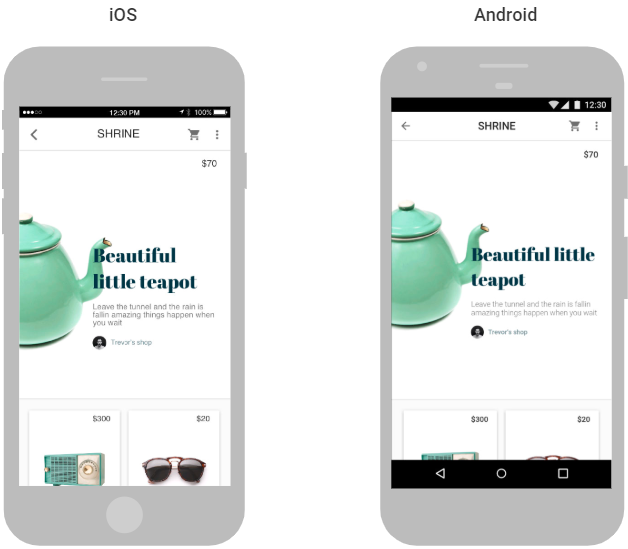
\includegraphics[width=9cm]{Images/chapter2/flutter_android_ios.png}
		\caption{{\footnotesize Ceci est une application de démonstration nommée Shrine\cite{noauthor_technical_nodate}}}
	\end{center}
\end{figure}

\tab Comme React Native, Flutter fournit également des vues de style réactif. Flutter adopte une approche différente pour éviter les problèmes de performances causés par la nécessité d'un pont JavaScript en utilisant un langage de programmation compilé, à savoir Dart. Dart est compilé «à l'avance» \acrshort{AOT} en code natif pour plusieurs plates-formes. Cela permet à Flutter de communiquer avec la plate-forme sans passer par un pont JavaScript qui effectue un changement de contexte. La compilation en code natif améliore également les temps de démarrage des applications.\medskip \\
\tab Flutter a une nouvelle architecture qui inclut des widgets qui ont l’air agréable, qui sont rapides, personnalisables et extensibles. il n'utilise pas les widgets de plate-forme (ou DOM WebViews), il fournit ses propres widgets.

\begin{figure}[h]
	\begin{center}
		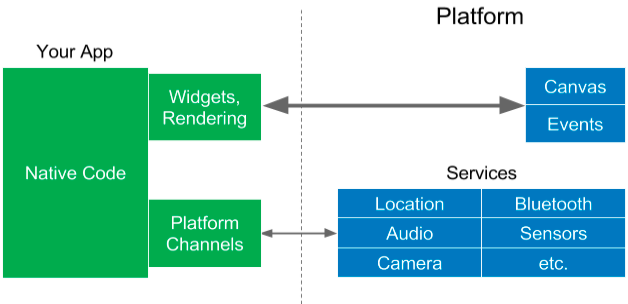
\includegraphics[width=11cm]{Images/chapter2/flutter.png}
		\caption{{\footnotesize Architecture du développement mobile a l'aide de Flutter\cite{leler_whats_2017}}}
	\end{center}
\end{figure}

\tab Flutter soulève les widgets et le moteur de rendu de la plateforme dans l'application, ce qui leur permet d'être personnalisables et extensibles. Tout ce que Flutter a besoin de la plate-forme est un canevas dans lequel les widgets doivent être rendus afin qu’ils puissent apparaître sur l’écran du périphérique, ainsi que l’accès aux événements (touches, minuteries, etc.) et aux services (localisation, caméra, etc.).\medskip \\
\tab Il existe toujours une interface entre le programme Dart (en vert) et le code de la plate-forme native (en bleu, pour iOS ou Android) qui effectue l’encodage et le décodage des données, mais cela peut être beaucoup plus rapide qu’un pont JavaScript.

\subsection{Pourquoi utiliser Flutter?}



\subsection{Principes de base}
\subsubsection{Tout est un Widget}


\section{Firebase}

\section{Google Maps}

\section{Google Books}